\documentclass[11pt]{article}
\usepackage[margin=1in]{geometry}
\usepackage{amsmath, amssymb}
\usepackage{graphicx}
\usepackage{float}
\usepackage{booktabs}
\usepackage[font=small,labelfont=bf]{caption}
\usepackage{subcaption}
\usepackage{hyperref}
\usepackage{enumitem}
\usepackage{xcolor}
\hypersetup{colorlinks=true,linkcolor=blue!60!black,urlcolor=blue!60!black}

\title{\Large\textbf{GAD vs Sella on HIP --- 3-method benchmark, tuned-Sella canonical}\\[4pt]
\normalsize 2026-04-28 v2 (revision of 04-28).
Transition1x train, 6 noise levels, 2000 steps, IRC = \texttt{sella\_hip}.}
\author{}
\date{}

\begin{document}
\maketitle
\thispagestyle{empty}

\paragraph{Canonical Sella in this revision = ``libdef'' tuning config}
($\delta_0{=}0.1$, $\gamma{=}0.4$). It dominates the previously-canonical
``default'' ($\delta_0{=}0.048$, $\gamma{=}0$) at 100/150/200\,pm by
+7--10\,pp. Tuning grid that established this is in the appendix
(§\ref{sec:sella_tune}); GAD-with-larger-$dt$ partial sweep also there
(§\ref{sec:gad_bigdt}).

\tableofcontents

\newpage
% =================================================================
\section{Headline}
% =================================================================

\begin{figure}[H]
\centering
\begin{subfigure}[t]{0.495\textwidth}
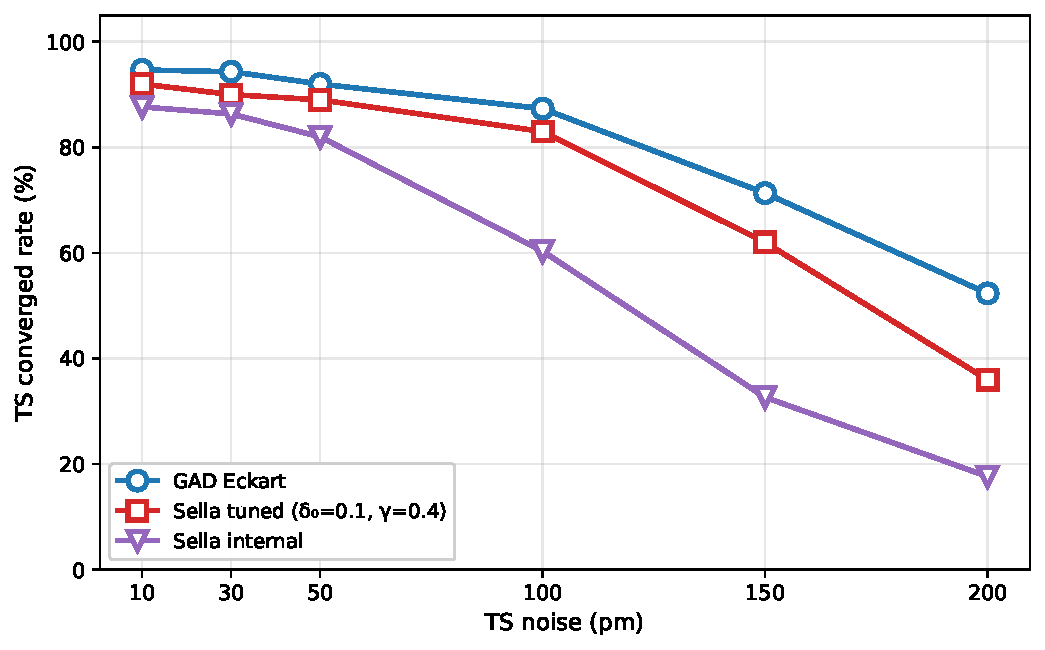
\includegraphics[width=\textwidth]{figures/fig_cmp_conv_3m_v2.pdf}
\caption{TS-converged rate vs.\ noise. GAD: $n{=}300$. Sella tuned: $n{=}100$. Sella internal: $n{=}300$.}
\end{subfigure}
\hfill
\begin{subfigure}[t]{0.495\textwidth}
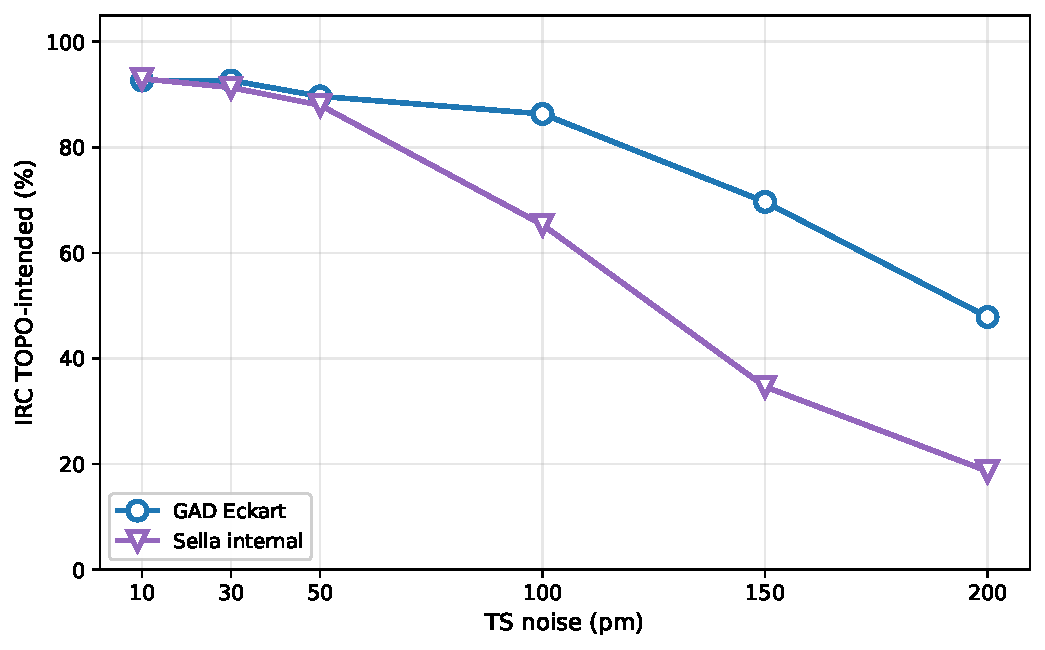
\includegraphics[width=\textwidth]{figures/fig_cmp_irc_topo_3m_v2.pdf}
\caption{IRC TOPO-intended rate vs.\ noise. ``Sella tuned'' line will appear
once IRC sweep on libdef pool lands (job 60003770).}
\end{subfigure}
\caption{TS-converged rate (left) and IRC TOPO-intended (right) for the
three canonical methods.}
\end{figure}

\begin{figure}[H]
\centering
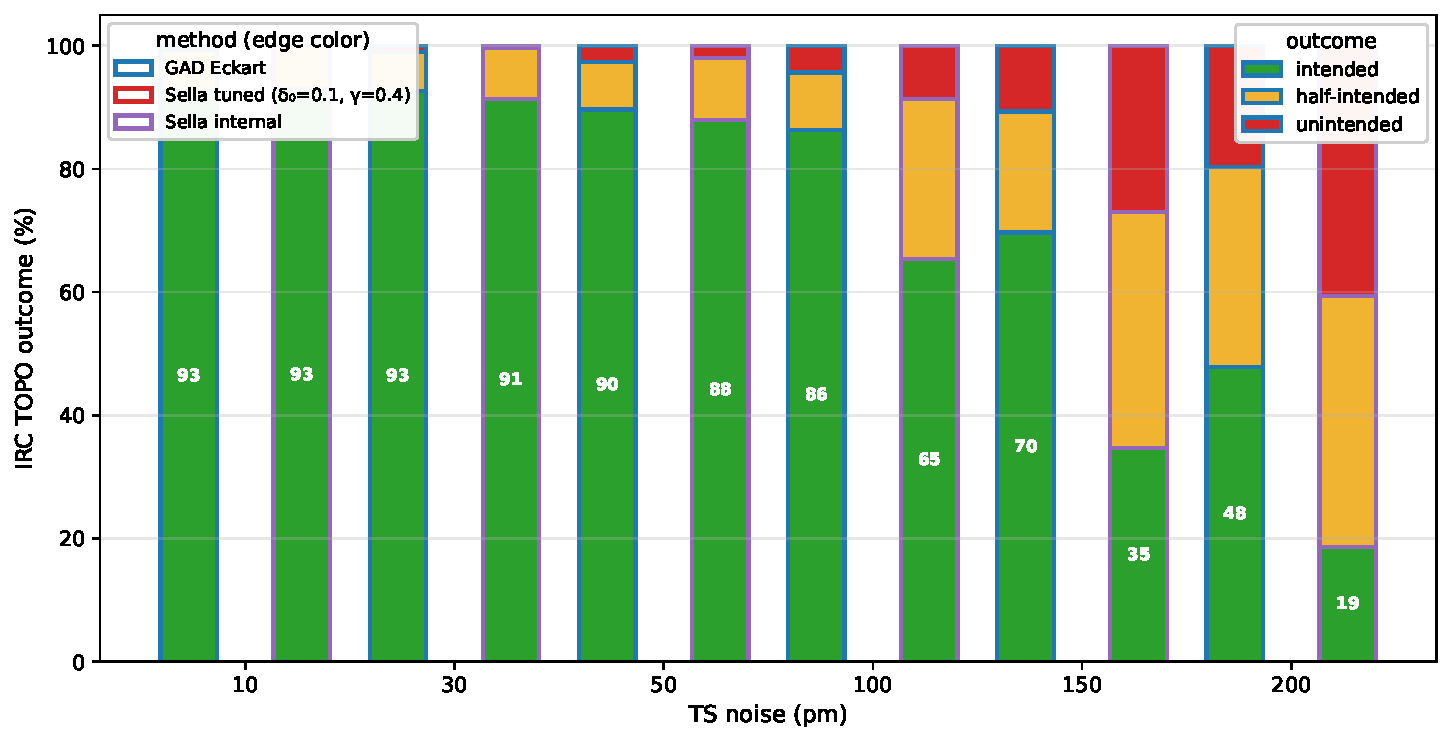
\includegraphics[width=\textwidth]{figures/fig_irc_intended_grouped_3m_v2.pdf}
\caption{IRC TOPO outcome breakdown per method per noise level.
Bar fill = outcome class (intended/half/unintended). Bar edge color =
method identity (matches Fig.~1).}
\end{figure}

\begin{center}
\textbf{TS-converged rate (\% by canonical criterion: $n_{\text{neg}}{=}1 \wedge f_{\max}{<}0.01$)} \\[0.3em]
\begin{tabular}{l|cccccc|c}
\toprule
Method & 10 & 30 & 50 & 100 & 150 & 200 & $n$ \\
\midrule
GAD Eckart (dt=0.003)         & 87.3 & 87.3 & 85.3 & 80.0 & 63.7 & 45.3 & 300 \\
\textbf{Sella tuned (libdef)} & 92.0 & 90.0 & 89.0 & \textbf{83.0} & \textbf{62.0} & \textbf{36.0} & 100 \\
Sella internal                & 87.7 & 86.3 & 82.0 & 60.3 & 32.7 & 17.0 & 300 \\
\bottomrule
\end{tabular}
\vskip0.8em
\textbf{IRC TOPO-intended rate (\%)} \\[0.3em]
\begin{tabular}{l|cccccc|c}
\toprule
Method & 10 & 30 & 50 & 100 & 150 & 200 & $n$ \\
\midrule
GAD Eckart (dt=0.003)         & 93.0 & 93.0 & 90.7 & 86.7 & 70.0 & 47.0 & 300 \\
Sella tuned (libdef)          & \multicolumn{6}{c|}{\emph{IRC sweep pending (job 60003770)}} & 100 \\
Sella internal                & 93.0 & 91.3 & 88.0 & 65.3 & 34.7 & 18.7 & 300 \\
\bottomrule
\end{tabular}
\end{center}

\newpage
% =================================================================
\section{GAD step-size over time}
\label{sec:gad_stepsize}
% =================================================================

\begin{figure}[H]
\centering
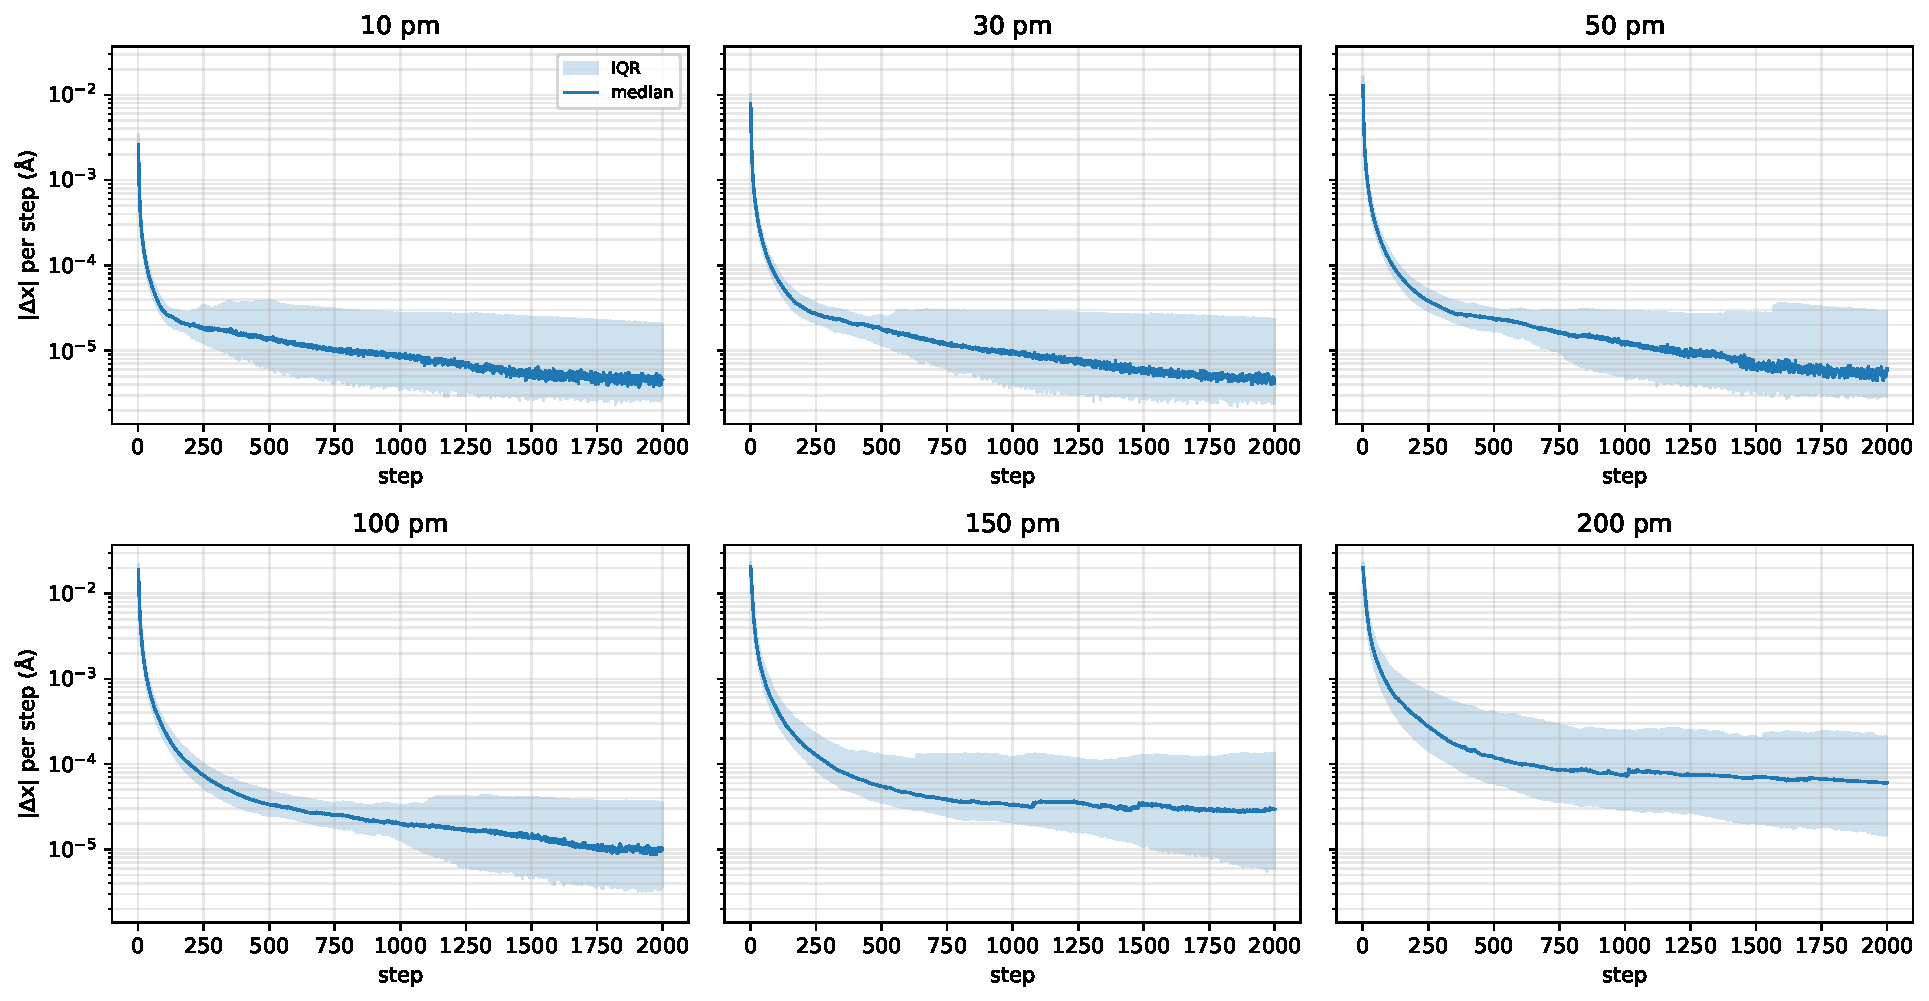
\includegraphics[width=\textwidth]{figures/fig_gad_stepsize_vs_step_v2.pdf}
\caption{GAD Eckart (dt=0.003) per-step Cartesian displacement (Å).
Median (line) and IQR (band), aggregated over 300 trajectories per
noise level. Sella step-size companion figure pending Sella traj-log
job 60002542.}
\end{figure}

\newpage
% =================================================================
\section{Appendix}
% =================================================================

\subsection{Sella tuning grid (full results, $n{=}100$)}
\label{sec:sella_tune}

\begin{figure}[H]
\centering
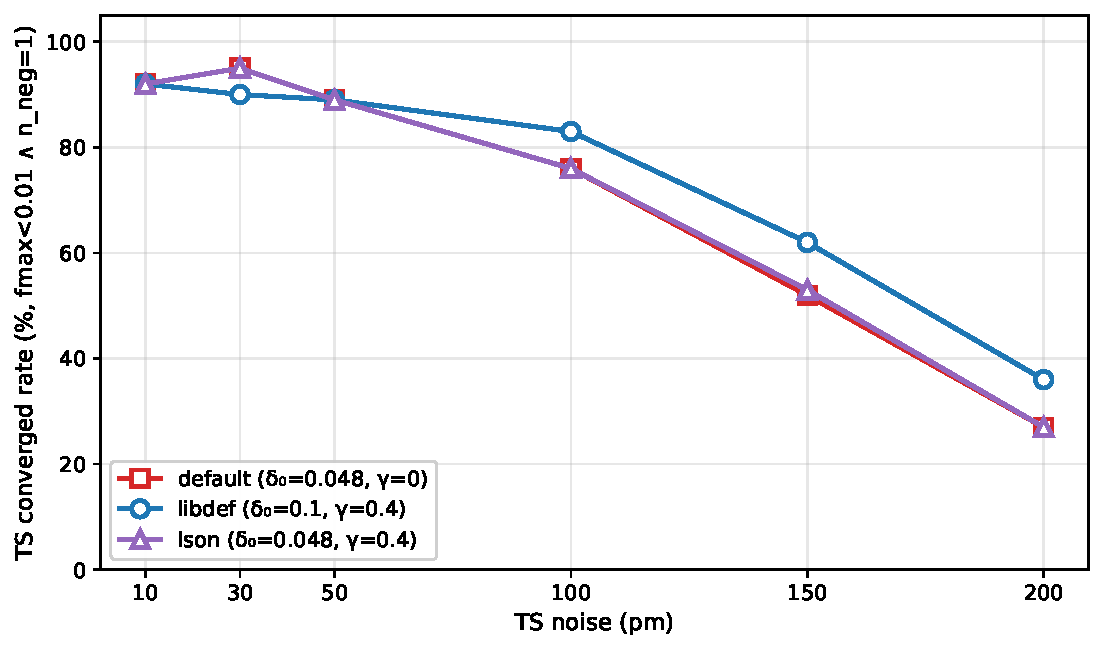
\includegraphics[width=0.92\textwidth]{figures/fig_sella_tune_grid.pdf}
\caption{Sella TS-converged rate as a function of two parameters:
$\delta_0$ (initial trust radius) and $\gamma$ (line search; $\gamma{=}0$
disables it). All cart+Eckart, $n{=}100$ samples per cell, fmax<0.01.}
\end{figure}

\begin{center}
\textbf{Sella tuning, TS-converged rate (\%, $n{=}100$ each)} \\[0.3em]
\begin{tabular}{l|cccccc|c}
\toprule
Config ($\delta_0$, $\gamma$) & 10 & 30 & 50 & 100 & 150 & 200 & mean nfev \\
\midrule
default (0.048, 0)            & 92.0 & \textbf{95.0} & 89.0 & 76.0 & 52.0 & 27.0 & 589 \\
\textbf{libdef (0.1, 0.4)}    & 92.0 & 90.0 & 89.0 & \textbf{83.0} & \textbf{62.0} & \textbf{36.0} & \textbf{502} \\
lson (0.048, 0.4)             & 92.0 & \textbf{95.0} & 89.0 & 76.0 & 53.0 & 27.0 & 585 \\
\bottomrule
\end{tabular}
\end{center}

Findings: (1) line search alone (\texttt{lson} vs \texttt{default}) is
inert; (2) larger trust radius (\texttt{libdef}) gains
+7--10\,pp at 100--200\,pm and is also \emph{cheaper} (502 vs 585--589
mean function evaluations) because larger trust → fewer steps;
(3) the only place where \texttt{libdef} loses is 30\,pm (90 vs 95) ---
small enough to potentially be sampling noise at $n{=}100$.

\subsection{GAD with larger $dt$ (partial)}
\label{sec:gad_bigdt}

Sweep in flight (job 59995949): three larger-$dt$ configs ($dt \in
\{0.005, 0.010, 0.020\}$) at 6 noise levels, $n{=}300$ each, fmax<0.01.
Motivated by §\ref{sec:gad_stepsize}: GAD per-step displacement at
$dt{=}0.003$ is $\sim10^{-3}$\,\AA, an order of magnitude below
Sella's QN trust step.

\begin{figure}[H]
\centering
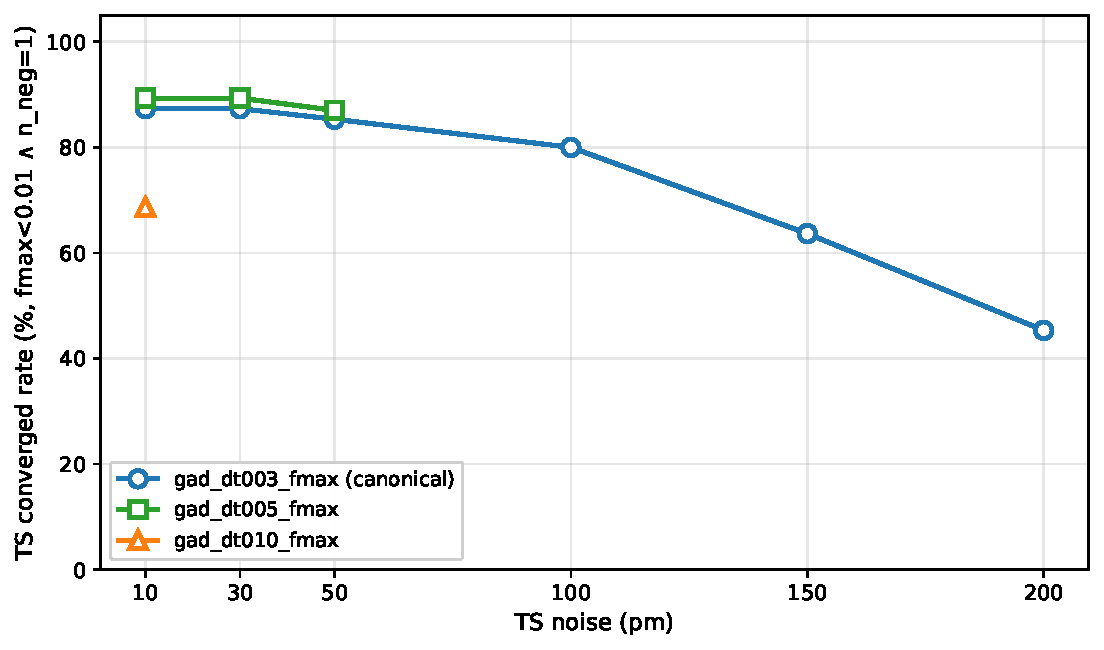
\includegraphics[width=0.92\textwidth]{figures/fig_gad_bigger_dt.pdf}
\caption{GAD TS-converged rate vs.\ noise for four step sizes.
Cells with no data: sweep still running.}
\end{figure}

\subsection{Data locations}

\begin{center}
\begin{tabular}{ll}
\toprule
Artifact & Path \\
\midrule
GAD Eckart canonical (dt=0.003)   & \texttt{runs/gad\_eckart\_fmax/} \\
GAD bigger-dt sweep (in flight)   & \texttt{runs/gad\_bigger\_dt/} \\
Sella tune grid                   & \texttt{runs/sella\_tune/\{default,libdef,lson\}/} \\
Sella tune IRC (in flight)        & \texttt{runs/irc\_sella\_libdef/} \\
Sella internal canonical          & \texttt{runs/sella\_2000/} \\
GAD IRC                           & \texttt{runs/irc\_sellahip\_allendpoints/} \\
Sella internal IRC                & \texttt{runs/irc\_sella\_int\_2000/} \\
This report                       & \texttt{IRC\_COMPREHENSIVE\_2026-04-28v2.tex/pdf} \\
\bottomrule
\end{tabular}
\end{center}

\subsection{In flight at write time}

\begin{itemize}[nosep,leftmargin=1.5em]
\item Job 59995949 (GAD bigger-$dt$, 18 tasks). Partial: $dt{=}0.005$ at 10/30/50\,pm; rest pending.
\item Job 60002542 (Sella traj-log, 3 configs $\times$ 1 noise, $n{=}50$). For Sella per-step displacement figure.
\item Job 60003770 (Sella libdef IRC, 6 noise $\times$ $n{=}100$). To populate canonical Sella IRC row.
\end{itemize}

\end{document}
